\model{Arrays}

An array variable stores a \emph{reference} to an array object.
We draw references as arrows, because they ``point'' to other memory locations.

\medskip
\begin{javalst}
    int[] data = null;


    int[] counts = {10, 3, 7, -5};


    double[] scores = new double[3];
\end{javalst}

\vspace{-9.75em}
\hfill 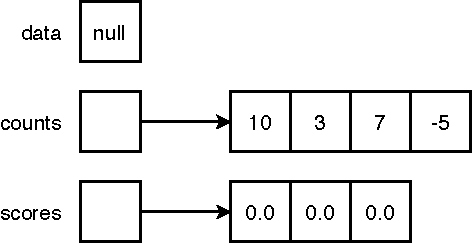
\includegraphics{diagram-array.pdf}
\hspace{2em} \null

\vspace{1.25em}
When passing an array to a method, only the reference is copied:

\medskip
\begin{javalst}
public static void printArray(int[] a) {
    System.out.print("{" + a[0]);
    for (int i = 1; i < a.length; i++) {
        System.out.print(", " + a[i]);
    }
    System.out.println("}");
}

public static void main(String[] args) {
    int[] nums = {159, 227};
    printArray(nums);
}
\end{javalst}

\vspace{-14em}
\hfill 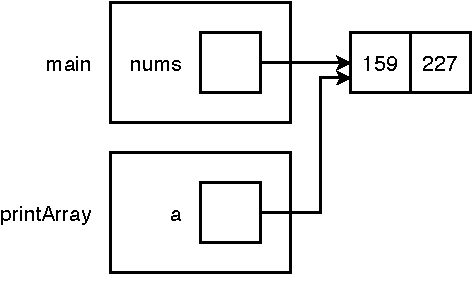
\includegraphics{diagram-array2.pdf}
\vspace{2em}


\quest{15 min}


\Q What is the length of each array?

\begin{multicols}{2}
\begin{enumerate}
\item \java{counts}? \ans[3em]{4}
\item \java{scores}? \ans[3em]{3}
\item \java{nums}?   \ans[3em]{2}
\item \java{a}?      \ans[3em]{2}
\end{enumerate}
\end{multicols}


\Q Looking at both diagrams above:

\begin{enumerate}
\item How many array variables were declared? \ans[3em]{5}
\item How many array objects were created? \ans[3em]{3}
\end{enumerate}


\Q Based on the top diagram, what is different about the variable named \java{data}?

\begin{answer}[3em]
The variable is \jans{null}, so there is no reference and no array object.
\end{answer}


\Q \label{key1}
Based on \java{counts} and \java{scores}, describe two ways that array objects can be created.
How are these two ways different from each other?

\begin{answer}[5em]
Arrays can be created either with curly braces or with the \jans{new} keyword.
The curly braces specify the initial values of array elements.
The \jans{new} keyword creates an array of specified length and initializes its elements to zero.
\end{answer}


\Q If the \java{printArray} method were to modify the array contents, would that change be visible in the \java{main} method?
Explain your reasoning.

\begin{answer}[3em]
Yes, because the variable \java{nums} and the variable \java{a} reference the same object.
\end{answer}


\Q Draw (or describe) a diagram of the following source code:

\begin{javalst}
int[] data = {1, 2, 3};
int[] copy = data;
\end{javalst}

\begin{answer}[15em]
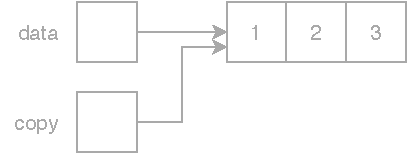
\includegraphics[scale=1]{data-copy.pdf}
\end{answer}


\Q (Optional) Paste the contents of \textit{Arrays.java} into \href{https://cscircles.cemc.uwaterloo.ca/java_visualize/#code=public+class+ClassNameHere+%7B%0A++++public+static+void+main(String%5B%5D+args)+%7B%0A++++++++%0A++++%7D%0A%7D&mode=edit&showStringsAsObjects=1}{Java Visualizer}.
What differences do you notice between the diagram in Java Visualizer and those in \ref{\currfilename}?

\begin{answer}
Answers might include:
\bull The variables are drawn in (method) frames.
\bull The array objects show the index of each cell.
\end{answer}
